\documentclass[11pt,a4wide]{article}
\usepackage[dvips]{graphicx}
\usepackage{mathrsfs}
\usepackage{amsfonts}
\usepackage{lscape}

\usepackage{epic,eepic}
\usepackage{amsmath}
\usepackage{amssymb}
\usepackage[dvips]{epsfig}
\usepackage[T1]{fontenc}
\usepackage{hyperref}
\usepackage{bezier}
\usepackage{pstricks}
\usepackage{dcolumn}% Align table columns on decimal point
\usepackage{bm}% bold math
%\usepackage{braket}
\usepackage[dvips]{graphicx}
\usepackage{pst-plot}
\usepackage{colortbl}
%\usepackage[english]{babel}
\usepackage{listings}
\usepackage{shadow}
\lstset{language=c++}
\lstset{basicstyle=\small}
%\lstset{backgroundcolor=\color{white}}
%\lstset{frame=single}
\lstset{stringstyle=\ttfamily}
%\lstset{keywordstyle=\color{red}\bfseries}
%\lstset{commentstyle=\itshape\color{blue}}
\lstset{showspaces=false}
\lstset{showstringspaces=false}
\lstset{showtabs=false}
\lstset{breaklines}

\newcommand{\One}{\hat{\mathbf{1}}}
\newcommand{\eff}{\text{eff}}
\newcommand{\Heff}{\hat{H}_\text{eff}}
\newcommand{\Veff}{\hat{V}_\text{eff}}
\newcommand{\braket}[1]{\langle#1\rangle}
\newcommand{\Span}{\operatorname{sp}}
\newcommand{\tr}{\operatorname{trace}}
\newcommand{\diag}{\operatorname{diag}}
\newcommand{\bra}[1]{\left\langle #1 \right|}
\newcommand{\ket}[1]{\left| #1 \right\rangle}
\newcommand{\element}[3]
    {\bra{#1}#2\ket{#3}}

\newcommand{\normord}[1]{
    \left\{#1\right\}
}


\usepackage{amsmath}





\begin{document}

\title{Project 1,  PHY981 Spring 2014}
%\author{}
\maketitle
\section*{Project 1, Deadline February 26}


We are going to study a schematic model (the Lipkin model, Nucl.
Phys. {\bf 62} (1965) 188) for the interaction among  $4$
fermions that can occupy two different energy levels. 
Although the model is simple, it contains several ingredients relevant for nuclear structure, from the handling
of angular momenta using lowering and raising operators, to  a typical diagonalization problem with close similarities
with shell-model calculations. The project ends also with a Hartree-Fock calculation. 
I would claim that if you understand the basic workings of this model, irrespective of its simplicity, you 
should be able to gain some of the underlying philosophy of how we interpret shell-model data.  
You can hand in your answer electronically (pdf, ps or scanned notes) or just your handwritten notes. 

The first part of the project involves a (slightly tedious) rewrite of various operators in terms of angular momentum 
operators. Here you need to play with various anti-commutation relations. The remaining part involves diagonalization of a $5\times 5$ Hamiltonian matrix, Hartree-Fock theory and discussion and analysis of your results.
There is also an optional part that gives you an additional score of 30\%. There the aim is to write a Hartree-Fock program which can be benchmarked against the closed form answers in exercise e). 
You are obviously free to collaborate with fellow students (I actually encourage that).  Good luck to you all! 

We have four fermions and 
each level has degeneration $d=4$. The two levels have quantum numbers $\sigma=\pm 1$,
with the upper level having  $\sigma=+1$ and energy
$\varepsilon_{1}=
\varepsilon/2$. The lower level  has $\sigma=-1$ and energy
$\varepsilon_{2}=-\varepsilon/2$. 
In addition, the substates  of each level are characterized  
by the quantum numbers $p=1,2,3,4$.  

We define the single-particle states
\[
\ket{u_{\sigma =-1,p}}=a_{-p}^{\dagger}\ket{0}
\hspace{1cm}
\ket{u_{\sigma =1,p}}=a_{+p}^{\dagger}\ket{0}.
\]
The single-particle states span an orthonormal basis.
The Hamiltonian of the system is given by
\[
\begin{array}{ll}
H=&H_{0}+H_{1}+H_{2}\\
&\\
H_{0}=&\frac{1}{2}\varepsilon\sum_{\sigma ,p}\sigma
a_{\sigma,p}^{\dagger}a_{\sigma ,p}\\
&\\
H_{1}=&\frac{1}{2}V\sum_{\sigma ,p,p'}
a_{\sigma,p}^{\dagger}a_{\sigma ,p'}^{\dagger}
a_{-\sigma ,p'}a_{-\sigma ,p}\\
&\\
H_{2}=&\frac{1}{2}W\sum_{\sigma ,p,p'}
a_{\sigma,p}^{\dagger}a_{-\sigma ,p'}^{\dagger}
a_{\sigma ,p'}a_{-\sigma ,p}\\
&\\
\end{array}
\]
where $V$ and $W$ are constants. The operator 
$H_{1}$ can move pairs of fermions as shown in Fig.~(a)
while $H_{2}$ is a spin-exchange term.
As shown in Fig.~(b),
$H_{2}$ moves a pair of fermions from a state $(p\sigma ,p' -\sigma)$ to a state
$(p-\sigma ,p'\sigma)$.
\begin{figure}[hbtp]
\includegraphics[width=1.0\textwidth]{fig1.ps}
\end{figure}\newline
\begin{enumerate}
\item[a)] Introduce the quasispin operators
\[
\begin{array}{ll}
J_{+}=&\sum_{p}
a_{p+}^{\dagger}a_{p-}\\
&\\
J_{-}=&\sum_{p}
a_{p-}^{\dagger}a_{p+}\\
&\\
J_{z}=&\frac{1}{2}\sum_{p\sigma}\sigma
a_{p\sigma}^{\dagger}a_{p\sigma}\\
&\\
J^{2}=&J_{+}J_{-}+J_{z}^{2}-J_{z}\\
&\\
\end{array}
\]
Show that these operators obey the commutation relations for angular momentum (you need to look up a textbook in quantum mechanics here or chapter 1 of Suhonen).\newline
\item[b)] Express $H$ in terms of the above quasispin operators and the number operator
\[
N=\sum_{p\sigma}
a_{p\sigma}^{\dagger}a_{p\sigma}.
\]
\item[c)] Show that $H$ commutes with $J^{2}$, viz., $J$ is a good quantum number.\newline
\item[d)] Consider thereafter a state with all four fermions in the lowest level (see the above figure).
We can write this state as
\[
\ket{\Phi_{J_z=-2}} =a_{1-}^{\dagger}a_{2-}^{\dagger}
a_{3-}^{\dagger}a_{4-}^{\dagger}\ket{0}.
\]
This state has $J_{z}=-2$ and belongs to the set of possible projections of 
$J=2$. We introduce the shorthand notation
$\ket{J,J_z}$ for states with different values of
spin $J$ and its projection $J_z$.

The other possible values are  $J_{z}=-1$, $J_{z}=0$, $J_{z}=1$
and $J_{z}=2$. 
Use the ladder operators
$J_{+}$ and $J_{-}$  to set up the states 
with spin $J_{z}=-1$ $J_{z}=0$, $J_{z}=1$
and $J_{z}=2$.  
The action of these operators on a state with given spin 
$J$ and $J_z$ is  (with $\hbar = 1$) 
\[
J_+\ket{J,J_z}=\sqrt{J(J+1)-J_z(J_z+1)}\ket{J,J_z+1}
\] 
and
\[
J_-\ket{J,J_z}=\sqrt{J(J+1)-J_z(J_z-1)}\ket{J,J_z-1},
\] respectively.
\newline
\item[e)] Use thereafter the quasispin operators to construct the Hamiltonian matrix 
$H$ for this five-dimensional space.  Find the eigenvalues
(numerically using for example python. If you need an eigenvalue solver for C++ or Fortran, let me know.)  for the following parameter sets:
\[
\begin{array}{cccc}
(1)&\varepsilon=2,&V=-1/3,&W=-1/4\\
(2)&\varepsilon=2,&V=-4/3,&W=-1
\end{array}
\]
Which state is the ground state? Comment and discuss your results.\newline
\item[f)]
The single-particle states for the 
 Lipkin model
\[
\ket{u_{\sigma =-1,p}}=a_{-p}^{\dagger}\ket{0}
\hspace{1cm}
\ket{u_{\sigma =1,p}}=a_{+p}^{\dagger}\ket{0}
\]
can now be used as basis for a new single-particle state
$\ket{\phi_{\alpha ,p}}$  via a unitary  transformation
\[
\ket{\phi_{\alpha ,p}}=
\sum_{\sigma =\pm1}C_{\alpha\sigma}\ket{u_{\sigma ,p}}
\]
with $\alpha=\pm 1$ og $p=1,2,3,4$. Why is $p$ the same in 
$\ket{\phi}$
as in $\ket{u}$?  Show that the new basis is orthonormal.\newline
\item[g)] With the new basis we can construct a new Slater determinant given by
$\ket{\Psi}$
\[
\ket{\Psi}=\prod_{p=1}^{4}b_{\alpha ,p}^{\dagger}\ket{0}
\]
with $b_{\alpha ,p}^{\dagger}\ket{0}=\ket{\phi_{\alpha ,p}}$. Use this Slater determinant to calculate
\[
E=\bra{\Psi}H\ket{\Psi},
\]
as a function of the coefficients $C_{\sigma\alpha}$. We assume that the coefficients are real.\newline
\item[h)] Show that
\[
  \frac{\epsilon}{3} > V+W,
\]
has to be fulfilled in order to find a minimum in the energy.
Hint: calculate the functional derivative  of the energy with respect to the coefficients $C_{\sigma\alpha}$. 

Discuss your results and give an interpretation of the Hartree-Fock results with respect to those obtained
by the exact diagonalization above. How would you interpret the Hartree-Fock results?

\item[g)] This exercise is optional, but gives you an additional score of 30\%.
The aim here is to build a Hartree-Fock program which solves the previous exercise numerically. In this case we have thus
results in a closed form which we can use to benchmark our program. Although this is a small problem, the program you end up writing
can be reused in later projects and for the final oral presentation as well. 
The Hartree-Fock algorithm can be broken down as follows. We recall that 
our Hartree-Fock matrix  is 
\[
\hat{h}_{\alpha\beta}^{HF}=\langle \alpha | \hat{h}_0 | \beta \rangle+
\sum_{j=1}^A\sum_{\gamma\delta} C^*_{j\gamma}C_{j\delta}\langle \alpha\gamma|V|\beta\delta\rangle_{AS}.
\]
Normally we assume that the single-particle basis $|\beta\rangle$ forms an eigenbasis for the operator
$\hat{h}_0$, meaning that the Hartree-Fock matrix becomes  
\[
\hat{h}_{\alpha\beta}^{HF}=\epsilon_{\alpha}\delta_{\alpha,\beta}+
\sum_{j=1}^A\sum_{\gamma\delta} C^*_{j\gamma}C_{j\delta}\langle \alpha\gamma|V|\beta\delta\rangle_{AS}.
\]
The Hartree-Fock eigenvalue problem
\[
\sum_{\beta}\hat{h}_{\alpha\beta}^{HF}C_{i\beta}=\epsilon_i^{\mathrm{HF}}C_{i\alpha},
\]
can be written out in a more compact form as
\[
\hat{h}^{HF}\hat{C}=\epsilon^{\mathrm{HF}}\hat{C}. 
\]

The Hartree-Fock equations are, in their simplest form, solved in an iterative way, starting with a guess for the
coefficients $C_{i\alpha}$. We label the coefficients as $C_{i\alpha}^{(n)}$, where the subscript $n$ stands for iteration $n$.
To set up the algorithm we can proceed as follows:
\begin{enumerate}
\item We start with a guess $C_{i\alpha}^{(0)}=\delta_{i,\alpha}$. Alternatively, we could have used random starting values as long as the vectors are normalized. Another possibility is to give states below the Fermi level a larger weight.
\item The Hartree-Fock matrix simplifies then to
\[
\hat{h}_{\alpha\beta}^{HF}=\epsilon_{\alpha}\delta_{\alpha,\beta}+
\sum_{j=1}^N\sum_{\gamma\delta} C^*_{j\gamma}^{(0)}C_{j\delta}^{(0)}\langle \alpha\gamma|V|\beta\delta\rangle_{AS}.
\]
Solving the Hartree-Fock eigenvalue problem yields then new eigenvectors $C_{i\alpha}^{(1)}$ and eigenvalues
$\epsilon_i^{\mathrm{HF}}^{(1)}$. 
\item With the new eigenvalues we can set up a new Hartree-Fock potential 
\[
\sum_{j=1}^N\sum_{\gamma\delta} C^*_{j\gamma}^{(1)}C_{j\delta}^{(1)}\langle \alpha\gamma|V|\beta\delta\rangle_{AS}.
\]
The diagonalization with the new Hartree-Fock potential yields new eigenvectors and eigenvalues.
This process is continued till for example
\[
\frac{\sum_{p} |\epsilon_i^{\mathrm{HF}}^{(n)}-\epsilon_i^{\mathrm{HF}}^{(n-1)}|}{m}\le \lambda,  
\]
where $\lambda$ is a user prefixed quantity ($\lambda \sim 10^{-8}$ or smaller) and $p$ runs over all calculated single-particle
energies and $m$ is the number of single-particle states.
\end{enumerate}
An example of a function in C++ which performs the Hartree-Fock calculation is shown here. In setting up your code you will need to write a function which sets up the single-particle basis, the expectation value of the one-body operator (called $h0$ in the function below) and the two-body matrix elements, called {\em matrixElement} below. You can use the code below or write your own. 
\begin{lstlisting}
void hartreeFock::run() {
    double interaction;
    // --------------- Setting up the HF-hamiltonian using C = 1 as guess, Armadillo is used for vectors
    mat H;
    vec E = zeros(nStates, 1);
    vec ePrev = zeros(nStates, 1);
    mat C = eye(nStates, nStates);
    vec diff;

    // Hartree-Fock loop
    int hfIt = 0;
    while (hfIt < HFIterations) {
        cout << "iteration = " << hfIt << endl;

        H = zeros(nStates, nStates);
        for (int alpha = 0; alpha < nStates; alpha++) {
            for (int gamma = 0; gamma < nStates; gamma++) {
                interaction = 0;
                for (int p = 0; p < nParticles; p++) {
                    for (int beta = 0; beta < nStates; beta++) {
                        for (int delta = 0; delta < nStates; delta++) {
                            interaction += C.at(p, beta) * C.at(p, delta) * matrixElement(alpha, beta, gamma, delta);
                        }
                    }
                }
                H(alpha, gamma) = H(gamma, alpha) = h0(alpha, gamma) + interaction;
            }
        }
        //Computing the HF one-body energies
        eig_sym(E, C, H);
        // Transposing the vectors
        C = trans(C);
        hfIt++;
        // Convergence test
        diff = E - ePrev;
        if (abs(diff.max()) < threshold)
            break;
        ePrev = E;
    }
    double E0 = calcEnergy(C);
    cout << "Final energy E = " << E0 << " after " << hfIt << " iterations, error < " << threshold << endl;
}
\end{lstlisting}

\end{enumerate}
\end{document}



